% =============================================================================
% appendix_body.tex: the Online Appendix. Read by appendix.tex (submitted as a
% separate, anonymized file) and by paper_wp.tex (appended to the working
% paper). Sections are lettered and exhibits numbered within them (Figure A1,
% Table B1, ...). Numbers come from the generated exhibits or from audit/*.rds,
% as in body.tex.
% =============================================================================

\section{Data and Measurement}\label{app:data}

The main outcome assigns road deaths to clock hours using the times recorded on their death certificates. Table~\ref{tab:measurement} summarizes the evidence on the reliability of this assignment: the correspondence between recorded crash and death times, the stability of reporting across abolition, the concentration of recorded times at whole and half hours, and the sensitivity of the estimates to shifted time windows and alternative treatments of rounded times. The subsections below describe each check.

\begin{table}[tbp]
  \caption{Measuring the Hour of Death}
  \label{tab:measurement}
  \centering\footnotesize\setlength{\tabcolsep}{5pt}
  \input{\tabdir/tab_measurement.tex}
  \begin{tablenotes}[Notes]
  Panels A and B use the death register only. Panel A: each federal highway crash with one death is paired with the only road-death certificate with a clock time in the same municipality on the same date. As a benchmark for chance, the crash is also paired with the certificates of the same municipality seven days later, which cannot record the same death. Panel B: linear triple difference on each share by state, season and window, weighted by deaths, with state-by-window, state-by-season and season-by-window effects. Panel D: equation~(\ref{eq:main}) for hour 0, one change per row; the window rows start the 60-minute window that many minutes before or after standard-time sunset; spread: full- and half-hour times spread over the 30 minutes around them; the last row takes sunset from the full NOAA solar algorithm \citep{meeus1998astronomical}. Standard errors clustered by state.
  \end{tablenotes}
  \begin{tablenotes}[Sources]
  \citet{datasus2025sim}; \citet{prf2025dados}.
  \end{tablenotes}
\end{table}

\subsection{The legal calendar}

The dates and states of DST come from the decrees themselves, typed from the texts published by the Presidency \citep{brasil2008decreto, brasil2017decreto, brasil2019decreto}. Under Decree 6,558/2008, DST ran from midnight on the third Sunday of October to midnight on the third Sunday of February, a week later when that Sunday was Carnival Sunday (as in 2012 and 2015); Decree 9,242/2017 moved the start to the first Sunday of November from 2018. Within the sample, DST therefore started between 15 October and 4 November and ended between 15 and 26 February. A day is under DST when the start date is on or before it and the end date is after it, since both changes happen at midnight. Decree 7,584/2011 added Bahia for 2011/12; Decree 7,826/2012 removed Bahia and added Tocantins for 2012/13, and Decree 8,112/2013 removed Tocantins. Decree 9,772/2019 abolished DST in the whole country and revoked the decrees still in force, 6,558/2008, 8,112/2013 and 9,242/2017 among them.

\subsection{Deaths on the road}

Road deaths are deaths whose underlying cause is a land-transport accident (ICD-10 V01--V89) and whose place of occurrence is a public road. Pedestrians are V01--V09; cyclists V10--V19; motorcyclists V20--V29; occupants of cars and light vehicles V40--V59; the remaining codes are other road users. The clock time is the time of death written on the certificate, in hours and minutes; times that are missing or invalid are left out of every hourly count. Figure~\ref{fig:records} shows, for the summer window, the share of land-transport deaths that occurred on the road and the share of road deaths without a valid clock time, by group and season. A linear triple difference on each share, computed by state, season and window and weighted by deaths, with state-by-window, state-by-season and season-by-window fixed effects, gives $+0.4$ percentage points (standard error 0.75) for the share on the road and $+0.4$ (0.65) for the share without a time (Table~\ref{tab:measurement}, Panel B). % record_integrity.rds, test.

The time on the certificate is close to the time of the crash for deaths at the scene. Pairing each federal highway crash with one death with the only road-death certificate with a clock time in the same municipality and on the same date gives 37,875 pairs, most of them the same event. The certificate's time minus the crash time has a median of zero minutes; it lies in the hour after the crash in 59.2 percent of the pairs and within 30 minutes either way in 66.9 percent. Pairs formed with the certificates of the same municipality seven days later, which cannot be the same event, give 4.7 and 5.2 percent (Table~\ref{tab:measurement}, Panel A). % record_integrity.rds, link.

Death certificates record legal clock time. If they recorded standard time, the profile of road deaths by clock hour in the treated states' summers under DST would sit one hour earlier than without DST. Net of the off-season and of the control states, the two profiles are closer with no shift (squared distance 7.8) than with a shift of one hour in either direction (17.1 and 24.5). % record_integrity.rds, clock.

\begin{figure}[tbp]
  \centering
  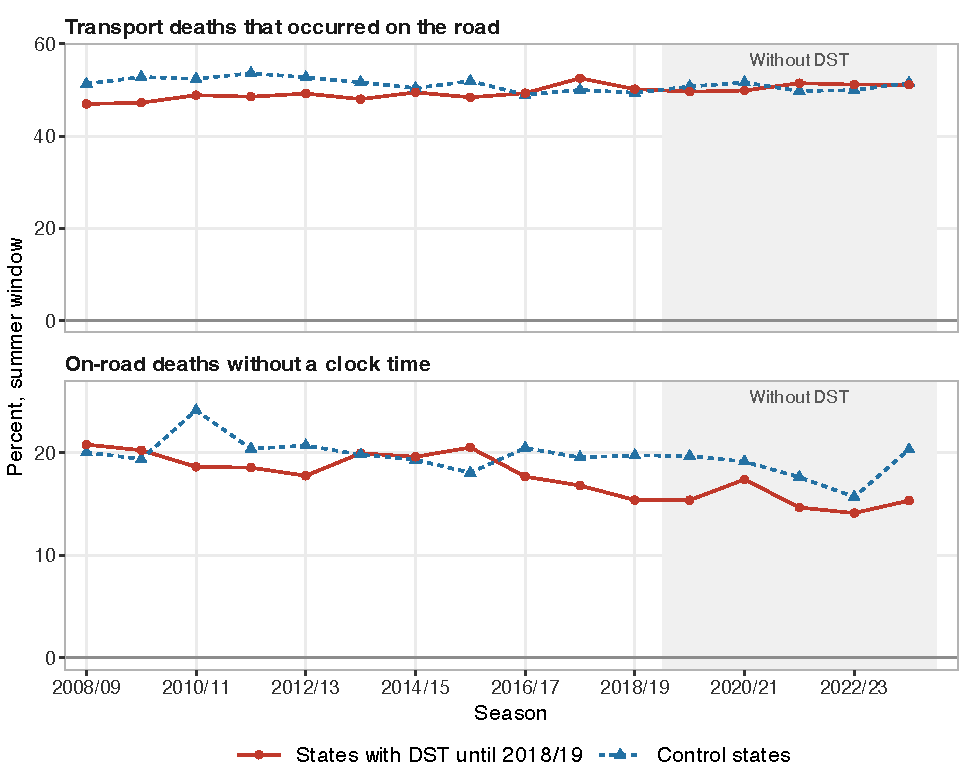
\includegraphics{fig_record_integrity.pdf}
  \caption{How Road Deaths Are Recorded}
  \label{fig:records}
  \begin{figurenotes}[Notes]
  Land-transport deaths (V01--V89) in the summer window. Top: share that occurred on the road rather than in hospital or elsewhere. Bottom: share of road deaths without a valid clock time.
  \end{figurenotes}
  \begin{figurenotes}[Source]
  \citet{datasus2025sim}.
  \end{figurenotes}
\end{figure}

\subsection{Federal highway crashes}

The PRF files have one row per crash from 2007 to 2025. Date formats, text encodings and the case of the light-phase labels change across years and are harmonized; a crash that appears on several rows differing only in a descriptive field is kept once. The municipality is given by name and is matched to the IBGE code within the state, with a table of alternative spellings and renamed municipalities typed by hand and checked against the coordinates that the PRF reports from 2017; every crash is matched. The light phase recorded by the officer is one of full daylight, dawn, dusk and night; in Panel B of Figure~\ref{fig:light} and in the first stage, dusk and night count as dark, and dawn crashes are left out. A second set of PRF files has one row per person in each crash, with the person's role, condition, sex and age \citep{prf2025pessoas}; matched to the crashes by their identifier, its dead match the deaths of the crash files to within one in every year of the sample, and it gives the sex and age of the dead in Table~\ref{tab:sex-age}.

\subsection{Traffic counts}

The counts are hourly vehicles by direction and vehicle class at continuous counting stations. A station-day enters only if all 24 clock hours are present and the daily total is positive. Each hourly count is assigned to the 60-minute bin, relative to standard-time sunset or sunrise at the station, that contains the midpoint of its clock hour. The flag for modeled values marks a station-day whose daily total equals exactly that of the same weekday one to four weeks earlier or later; such repetitions are absent from counts before June 2019 and frequent after it at the stations whose published values DNIT estimated. Of the stations in the 23 states of the sample, 247 report only before abolition and 315 only after. % EXPLICANDO_O_PROJETO.md, section 3.3 (count corrected in the code audit of 09/10/2026).

The stations record legal clock time. If they recorded standard time, the profile of traffic by clock hour in the treated states' summers under DST would sit one hour earlier than without DST. Net of the off-season and of the control states, the two profiles are closer with no shift (squared distance 0.23) than with a shift of one hour in either direction (0.32 and 0.38). % traffic_volume.rds, clock.

\subsection{Sun times and recorded times}

Sunrise and sunset are computed at the municipal seat \citep{noaa2025solar}, with the seat coordinates from IBGE (2010 seats; a point inside the 2020 boundary for the five municipalities created in 2013) and the standard offset of each municipality's legal time zone \citep{brasil1913decreto, brasil2008lei, brasil2013lei}. Recorded clock times heap: 34.5 percent of road deaths are recorded on the full hour and 23.0 percent on the half hour, and 90 percent on a multiple of five minutes (21.3, 19.4 and 95.2 percent for federal highway deaths). % heaping.rds, heap_share.
Because hour 0 is defined relative to the sunset of each municipality and date, a heap at, say, 7:00 p.m.\ falls inside or outside hour 0 depending on the place and the date. Figure~\ref{fig:window-shift} and Panel D of Table~\ref{tab:measurement} show the estimates when the window is moved by up to 15 minutes, when sunset comes from NOAA's full solar algorithm \citep{meeus1998astronomical} instead of the general equations, when every time recorded on the full or half hour is spread evenly over the 30 minutes around it, and when those times are dropped.

% -----------------------------------------------------------------------------
\section{Additional Results}\label{app:results}

\subsection{Other windows, samples and clocks}

\begin{figure}[tbp]
  \centering
  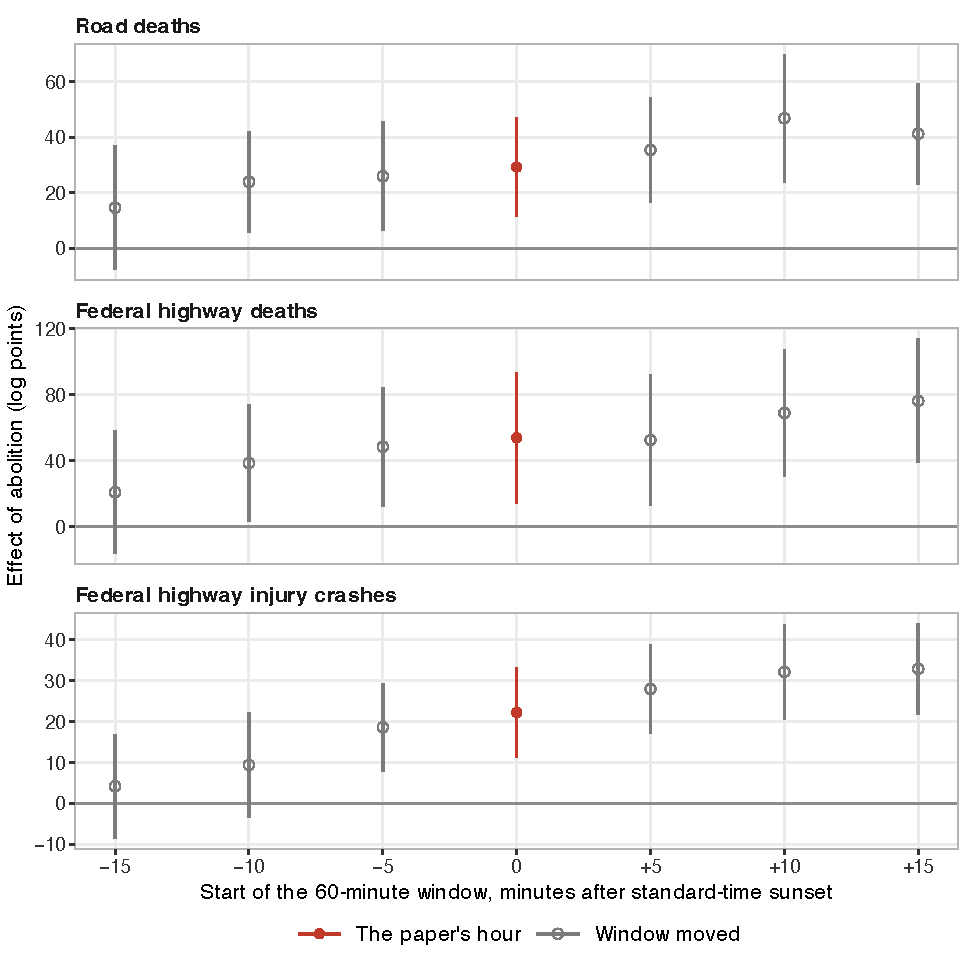
\includegraphics{fig_window_shift.pdf}
  \caption{The Hour after Sunset, Moved Earlier and Later}
  \label{fig:window-shift}
  \begin{figurenotes}[Notes]
  Each point is equation~(\ref{eq:main}) for a 60-minute window that starts the stated number of minutes after standard-time sunset; 0 is hour 0 of Table~\ref{tab:main}. 95 percent confidence intervals, standard errors clustered by state.
  \end{figurenotes}
  \begin{figurenotes}[Sources]
  \citet{datasus2025sim}; \citet{prf2025dados}.
  \end{figurenotes}
\end{figure}

\begin{figure}[tbp]
  \centering
  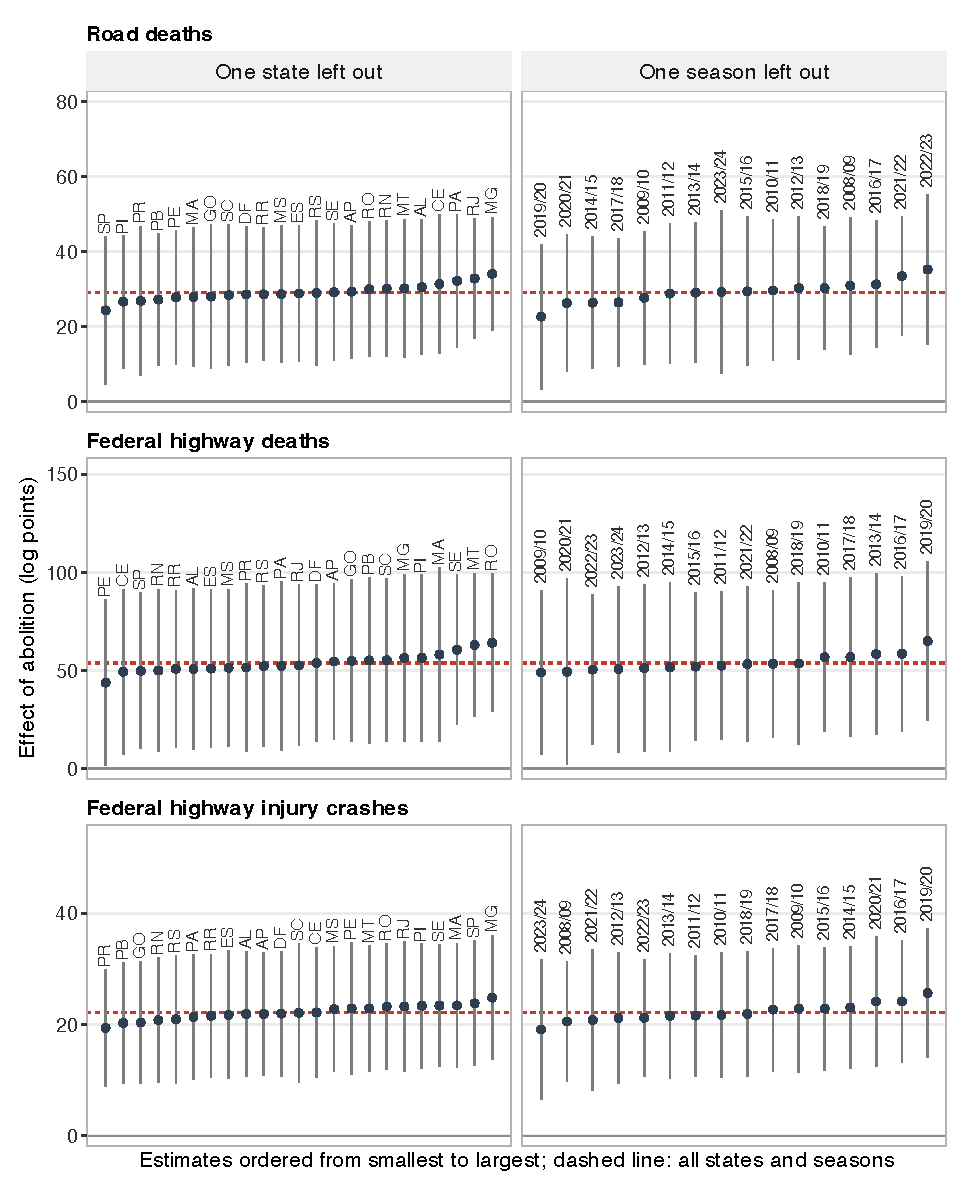
\includegraphics{fig_leave_out.pdf}
  \caption{Leaving One State or One Season Out}
  \label{fig:leave-out}
  \begin{figurenotes}[Notes]
  Equation~(\ref{eq:main}) for hour 0, dropping the state or season named above each point. 95 percent confidence intervals, standard errors clustered by state; the dashed line is the estimate with every state and season.
  \end{figurenotes}
  \begin{figurenotes}[Sources]
  \citet{datasus2025sim}; \citet{prf2025dados}.
  \end{figurenotes}
\end{figure}

\begin{table}[tbp]
  \caption{The Hour after Sunset under Other Samples}
  \label{tab:sensitivity}
  \centering\footnotesize\setlength{\tabcolsep}{5pt}
  \input{\tabdir/tab_sensitivity.tex}
  \begin{tablenotes}[Notes]
  Equation~(\ref{eq:main}) for hour 0, one change per row, standard errors clustered by state. Panel A: the coast row drops the events in the 279 municipalities that face the sea \citep{ibge2022defrontantes}; the holiday row drops Saturday before Carnival to Ash Wednesday and 24 December to 1 January. The summer-window rows are the difference in differences of Table~\ref{tab:robustness} with separate effects for the first two and the last three summers without DST. The rows without March 2020 to February 2022 have separate effects for 2019/20 and for 2022/23 and 2023/24. Panel B: the rain share is the share of the state's municipalities, weighted by their road deaths before abolition, with at least 1 mm of rain that day at the municipal seat \citep{xavier2022new}; as a control, and interacted with every term of equation~(\ref{eq:main}), which gives the effect on a dry state-day and its change on a fully rainy one. Panel C: one model with separate effects for the school weeks (15 November to 7 December), the school holidays (24 December to 15 January) and the other days of the summer window, and state effects for each part; 2020/21, with remote classes and school years extended into 2021, counts among the other days. The holiday split has separate effects for 24 December to 1 January and 2 to 15 January. The placebo uses only the seasons before abolition and treats 2014/15 to 2018/19 as if after it.
  \end{tablenotes}
  \begin{tablenotes}[Sources]
  \citet{datasus2025sim}; \citet{prf2025dados}.
  \end{tablenotes}
\end{table}

Moving the window changes the estimate in the direction light predicts: a window that starts 15 minutes before standard-time sunset includes minutes that were light in both regimes and gives 14.6 log points for road deaths, and one that starts 15 minutes after it is darker throughout and gives 41.2 (Figure~\ref{fig:window-shift}). Spreading the times recorded on the full or half hour gives 31.4 (9.5), and dropping them 16.7 (12.9), with less than half the deaths in hour 0 (Table~\ref{tab:measurement}). Leaving out one state at a time keeps the estimate for road deaths between 24.3 (without S\~ao Paulo) and 34.1 (without Minas Gerais), and one season at a time between 22.7 (without 2019/20) and 35.2 (without 2022/23) (Figure~\ref{fig:leave-out}). With the Northeast alone as the control group the estimate is 32.9 (9.2); with the four states of the North alone, 15.7 (8.8). Dropping the three La Ni\~na summers of 2020/21 to 2022/23 gives 43.5 (9.5), dropping Carnival and the year-end holidays 30.8 (8.0), and dropping the 279 municipalities that face the sea, where summer trips to the beach go, 36.3 (9.4) (Table~\ref{tab:sensitivity}).

Most of the summer window falls in the school holidays. In the calendars of the state school networks we found, classes ran from 15 November to at least 7 December and did not run from 24 December to 15 January. The latest end was 23 December and the earliest return 16 January, in Goi\'as, the one state network that returns in January; elsewhere classes resume in February \citep{saopaulo2018resolucao, goias2018parecer, minas2023ano}. The exception is Par\'a, a control state, whose 2019 school year ran from 11 March 2019 to 30 January 2020 \citep{para2018calendario}. Municipal and private schools set their own calendars within the 200 school days the law requires, and can differ by a few days; in Goi\'as, private schools proposed ending the 2019 year on 11 or 14 December \citep{goias2018parecer}.

Panel C of Table~\ref{tab:sensitivity} estimates one model with separate effects for the school weeks, the school holidays and the other days of the summer window. Road deaths in hour 0 rose by 58.1 log points (12.6) in the school weeks and by $-12.3$ (16.8) in the holidays. The holidays contain Christmas, the New Year and the summer trips, but none of them accounts for the difference. Split again, the holidays show 5.8 (28.7) from 24 December to 1 January and $-27.9$ (19.0) from 2 to 15 January, after the year-end festivities. Without the 279 municipalities on the coast, where the beach trips go, the difference between the school weeks and the holidays is 66.6 (22.1); without Par\'a, 73.7 (21.3). Before abolition, the two parts of the window moved alike: repeating the split on the seasons before 2019, as if abolition had come in 2014/15, gives a difference of $-15.9$ (26.2). Trips inland, which leave from the same states, cannot be separated this way. On federal highways the estimates for deaths are positive in both parts and imprecise, and injury crashes rose about equally in both. Section~\ref{sec:transitions} of the paper uses the school weeks to compare abolition with the clock changes, which fall in term time.

\begin{figure}[tbp]
  \centering
  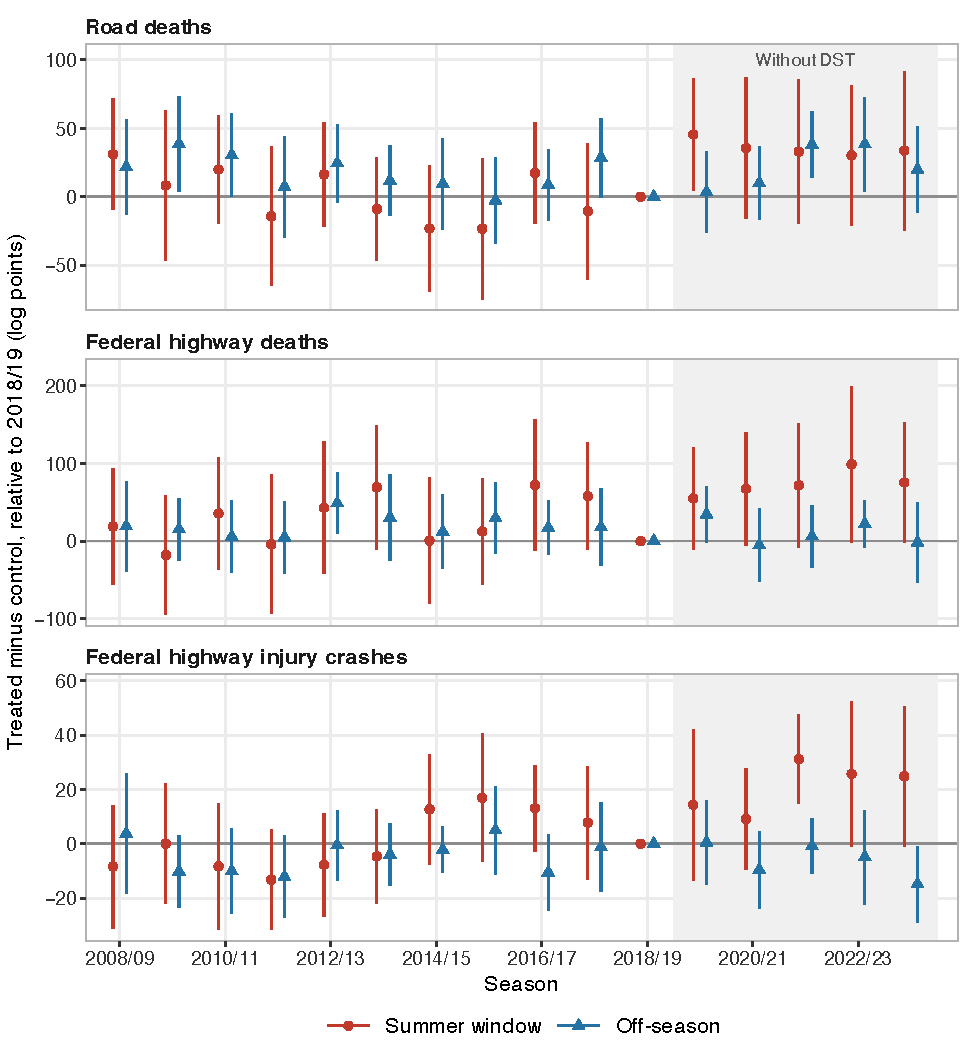
\includegraphics{fig_window_legs.pdf}
  \caption{The Two Legs of the Triple Difference, Season by Season}
  \label{fig:window-legs}
  \begin{figurenotes}[Notes]
  Hour after standard-time sunset. Each point is the coefficient on the treated states in one season from a Poisson model of the summer window alone or of the off-season alone, with state and date effects, against 2018/19. Up to its common date effects, the triple difference is the summer coefficient minus the off-season coefficient; Figure~\ref{fig:event-study} shows it against the average season with DST rather than 2018/19. 95 percent confidence intervals, standard errors clustered by state.
  \end{figurenotes}
  \begin{figurenotes}[Sources]
  \citet{datasus2025sim}; \citet{prf2025dados}.
  \end{figurenotes}
\end{figure}

Figure~\ref{fig:window-legs} shows where the season-to-season swings of the triple difference come from. In the summer window, the gap between treated and control states in hour 0 rose with abolition and stayed at about the same level in all five seasons without DST. In the off-season, which has no change of light, the gap was low in 2019/20, whose off-season includes April to June 2020, and high in 2021/22 and 2022/23. The larger triple-difference estimates of the first two seasons therefore come from the off-season leg. In the summer window alone, the first two summers give 39.3 (12.4) and the last three 31.2 (15.8). Without any day from March 2020 to February 2022, the triple difference gives 36.9 (19.4) for 2019/20 and 18.7 (11.3) for the last two summers.

\subsection{State-by-day fixed effects and sensitivity to trends}

\begin{figure}[tbp]
  \centering
  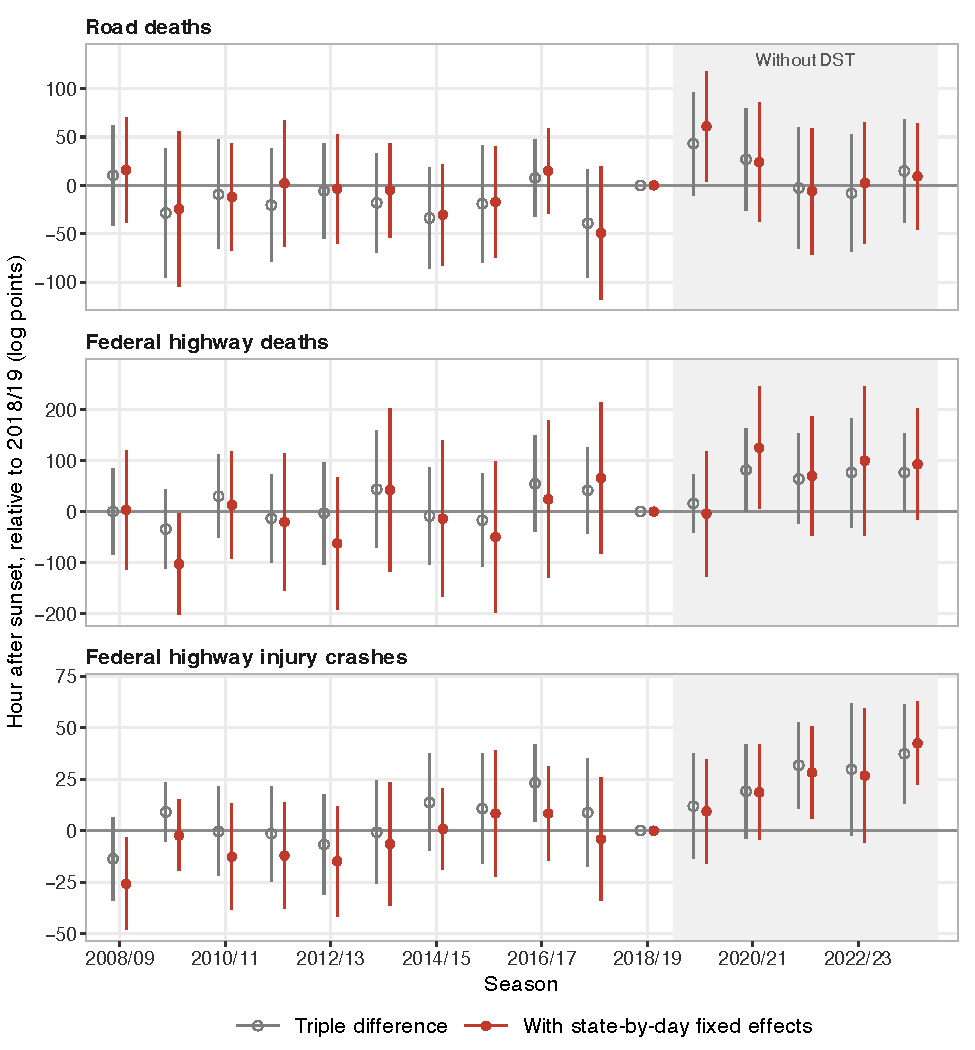
\includegraphics{fig_within_day.pdf}
  \caption{The Hour after Sunset with State-by-Day Fixed Effects}
  \label{fig:within-day}
  \begin{figurenotes}[Notes]
  Grey: hour 0 in Figure~\ref{fig:event-study}. Red: the same hour estimated against hours 3 to 5 before and 2 to 4 after sunset of the same state and day, with state-by-day fixed effects and the fixed effects of equation~(\ref{eq:main}) interacted with the hour. Both against the average of the seasons with DST, as in Figure~\ref{fig:event-study}. 95 percent confidence intervals, standard errors clustered by state.
  \end{figurenotes}
  \begin{figurenotes}[Sources]
  \citet{datasus2025sim}; \citet{prf2025dados}.
  \end{figurenotes}
\end{figure}

Figure~\ref{fig:within-day} repeats the event study with a fixed effect for every state and day, which absorbs any shock common to all hours of a state's day, such as rain, a holiday or the volume of traffic. Pooled over the seasons after abolition, the estimate for road deaths is 27.7 log points (12.4; Table~\ref{tab:robustness}); the standard error does not fall, because the noise in a single hour's count is sampling noise rather than daily shocks.

\begin{table}[tbp]
  \caption{Within the Day, Treated and Control States Each Alone}
  \label{tab:within-group}
  \centering\footnotesize
  \input{\tabdir/tab_within_group.tex}
  \begin{tablenotes}[Notes]
  Hour 0 against hours of the same state and day whose light did not change (evening: 3 to 5 hours before and 2 to 4 after standard-time sunset; morning: 2 to 4 hours before and after standard-time sunrise), summer window against off-season, after abolition against before, estimated in each group separately with state-by-day effects and the fixed effects of equation~(\ref{eq:main}) interacted with the hour; the hours in between, whose light changed in part, have their own coefficients. Column 4: vehicles at federal highway count stations, with station-by-day and station-by-hour effects. Standard errors clustered by state.
  \end{tablenotes}
  \begin{tablenotes}[Sources]
  \citet{datasus2025sim}; \citet{prf2025dados}; \citet{dnit2025pnct}.
  \end{tablenotes}
\end{table}

The control states kept their clocks, but schedules set on Bras\'ilia time, such as national broadcasts, ran an hour earlier on those clocks in every summer with DST and have run at the same clock time all year since. If that change moved the control states' evening, they would not supply the counterfactual the triple difference assumes. Table~\ref{tab:within-group} compares hour 0 with hours of the same state and day whose light did not change, in each group alone. Traffic did not move in the control states' evening: vehicles in hour 0 changed by $-0.2$ log points (0.7), against $-5.4$ (1.6) in the treated states. Road deaths in the control states' hour 0 did rise relative to the rest of their day, by 19.7 log points (6.5), while their federal highway deaths and injury crashes in that hour fell. Whatever raised those deaths did not move traffic. To the extent that it came from the control states' own schedules, the triple difference understates the effect: within the treated states alone, road deaths in hour 0 rose by 47.2 log points (7.8). In the morning, road deaths in hour 0 fell in both groups and traffic rose in both, so the triple difference nets out a change the control states share. Within the treated states alone, road deaths in the morning hour that turned light fell by 19.4 log points (9.6). Applied to the 107 and 110 deaths per summer the two hours had before abolition, that fall offsets less than a third of the evening rise.

\begin{figure}[tbp]
  \centering
  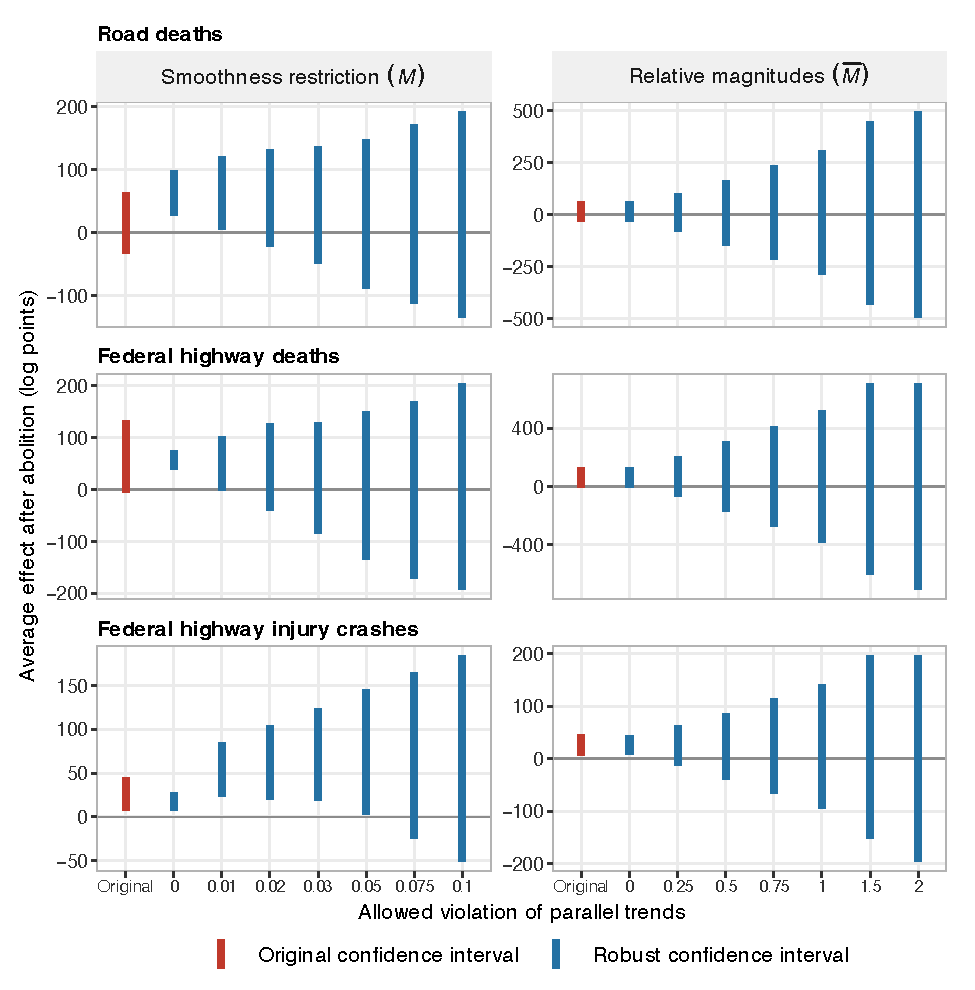
\includegraphics{fig_honestdid.pdf}
  \caption{Sensitivity to Violations of Parallel Trends}
  \label{fig:honestdid}
  \begin{figurenotes}[Notes]
  95 percent confidence intervals for the average of the five season coefficients after abolition in Figure~\ref{fig:event-study}, hour 0 \citep{rambachan2023more}. These coefficients are measured against 2018/19, not against the average of the seasons before abolition, so the target differs from $\beta$ in Table~\ref{tab:main}. Left: the slope of the violation may change by at most $M$ between seasons, in log units (0.01 is 1 log point). Right: the violation after abolition is at most $\bar M$ times the largest one before it.
  \end{figurenotes}
  \begin{figurenotes}[Sources]
  \citet{datasus2025sim}; \citet{prf2025dados}.
  \end{figurenotes}
\end{figure}

Figure~\ref{fig:honestdid} reports the sensitivity analysis of \citet{rambachan2023more} for the average post-abolition coefficient of the event study. The method measures the violations of parallel trends from a single reference season, so here the coefficients are taken against 2018/19, not against the average season with DST as in Figure~\ref{fig:event-study}. For road deaths that average is 14.8 log points, and its conventional interval already includes zero, because a single reference season is a noisy baseline. If the pre-abolition trend is extended linearly ($M=0$), the interval is 28 to 99 log points; allowing its slope to change by 0.02 per season (2 log points) brings zero into it. % honestdid.rds.
The event study therefore cannot rule out departures from parallel trends of the size of its own season-to-season noise, which is why the paper's case rests on the pattern within the day.

\subsection{Who dies}

\begin{table}[tbp]
  \caption{Who Dies in the Hour That Turned Dark}
  \label{tab:road-users}
  \centering\footnotesize\setlength{\tabcolsep}{5pt}
  \input{\tabdir/tab_road_users.tex}
  \begin{tablenotes}[Notes]
  Road deaths in hour 0, equation~(\ref{eq:main}) estimated separately for each group, standard errors clustered by state. Road users from the ICD-10 block of the underlying cause (Appendix~\ref{app:data}); 85 percent of the other road users who died in hour 0 have no vehicle specified (V87 to V89), 10 percent were in heavy transport vehicles and the rest in buses, three-wheeled or other vehicles. Weekends and holidays: Saturdays, Sundays and national holidays (fixed dates, Carnival Monday and Tuesday, Good Friday); the last row of Panel C also drops the Saturday before Carnival to Ash Wednesday and 24 December to 1 January. Dashes: fewer than five deaths per summer in the treated states before abolition, too few to estimate.
  \end{tablenotes}
  \begin{tablenotes}[Source]
  \citet{datasus2025sim}.
  \end{tablenotes}
\end{table}

Table~\ref{tab:road-users} splits road deaths in hour 0 by road user, by the age and sex of pedestrians, and by type of day. Among pedestrians, deaths of those aged 15 to 64, two thirds of the total, rose by 91.1 log points (30.9); the other age groups are too small to estimate. Motorcyclists rise by 19.6 (10.9); the estimate for car occupants is close to zero and imprecise ($-0.2$, 35.2); the residual group, mostly deaths with no type of vehicle recorded, rises by 55.8 (26.4). The estimate on weekends and holidays (41.3, 15.8) is larger than on working days (16.1, 10.0), and stays so without Carnival and the year-end holidays (39.3, 16.2).

\begin{table}[tbp]
  \caption{Sex and Age of the Dead in the Hour That Turned Dark}
  \label{tab:sex-age}
  \centering\footnotesize\setlength{\tabcolsep}{3pt}
  \input{\tabdir/tab_sex_age.tex}
  \begin{tablenotes}[Notes]
  Equation~(\ref{eq:main}) for hour 0, estimated separately for the dead of each sex and age group, standard errors clustered by state. Road deaths: sex and age from the death certificate. Federal highway deaths: sex and age from the police record of each person in the crash; the age of 12 percent of the dead is not recorded before 2017 and of 6 percent from 2017, when the record began to enter a missing age as zero, which is treated as not recorded. Deaths per summer: mean in the treated states' summer window before abolition. Dashes: fewer than five deaths per summer, too few to estimate.
  \end{tablenotes}
  \begin{tablenotes}[Sources]
  \citet{datasus2025sim}; \citet{prf2025dados, prf2025pessoas}.
  \end{tablenotes}
\end{table}

Table~\ref{tab:sex-age} splits the dead in hour 0 by sex and age in both registers. Men are about four fifths of the dead in both. Their road deaths rose by 33.8 log points (9.9) and their federal highway deaths by 65.2 (20.7); the estimates for women, 12.7 (22.2) and 5.8 (42.3), are too imprecise to say whether their deaths rose less. Every age group from 15 years on has a positive estimate in road deaths, and so does every group on federal highways with enough deaths to estimate. Their intervals overlap too much to rank them.

\subsection{Traffic volume and risk per vehicle}

\begin{table}[tbp]
  \caption{Traffic Volume and Risk per Vehicle on Federal Highways}
  \label{tab:volume}
  \centering\footnotesize
  \input{\tabdir/tab_traffic_volume.tex}
  \begin{tablenotes}[Notes]
  Log points, standard errors clustered by state in parentheses, permutation p-values in brackets. Column 1: equation~(\ref{eq:main}) on hourly vehicle counts at continuous counting stations, with station fixed effects; summers 2014/15 to 2018/19 and 2021/22 to 2024/25. Column 2: the 30 pairs formed by a station counted only after abolition within 2 km of one counted only before on the same highway, with pair-by-window and pair-by-season effects in place of the state effects. Columns 3 and 5: as in Table~\ref{tab:main}, on the same summers as column 1. Per vehicle: crash or death estimate minus the volume estimate of column 1. Every column is re-estimated with the same random set of 11 treated states in each of 999 draws, so the per-vehicle columns have their own reference distribution; permutation tests are on t-statistics, a per-vehicle difference divided by the square root of the sum of its two squared standard errors.
  \end{tablenotes}
  \begin{tablenotes}[Sources]
  \citet{dnit2025pnct}; \citet{prf2025dados}.
  \end{tablenotes}
\end{table}

Table~\ref{tab:volume} reports, for the seven hours around sunset and sunrise, the triple difference on hourly vehicle counts at federal highway stations (column 1), on federal highway injury crashes and deaths (columns 3 and 5), and their difference, the change per vehicle (columns 4 and 6). Because no station is counted both before and after abolition, the volume model has station fixed effects and the seasonal comparison runs at the level of the state, as in equation~(\ref{eq:main}). Column 2 follows the 30 stations that were moved at most 2 kilometers along the same highway, as pairs: the evening falls are smaller there and the morning rise larger. The crash columns come from the same summers as the volume, on which hour 0 shows no pre-abolition trend in injury crashes. Section~\ref{sec:traffic} of the paper discusses hour 0, the hour before sunset and the hour after sunrise.

\subsection{Rain and street lighting}

On a rainy, overcast evening the hour was already dim under DST, so abolition should darken it less. Panel B of Table~\ref{tab:sensitivity} points that way for every outcome, without precision: for road deaths, the effect on a dry state-day is 43.5 log points (15.5) and the change from a dry to a fully rainy state-day $-4.3$ (34.4). Controlling for the share of the state under rain leaves the main estimate at 29.1.

\begin{table}[tbp]
  \caption{Street Lighting}
  \label{tab:lighting}
  \centering\footnotesize
  \input{\tabdir/tab_street_lighting.tex}
  \begin{tablenotes}[Notes]
  Municipalities split within each state at the median, weighted by road deaths before abolition, of the share of households on a street face without public lighting: Census 2022 in Panels A and B, urban tracts of Census 2010 in Panel C. The municipality that crosses the median goes to the darker half; the Federal District, a single municipality, falls wholly in it. Equation~(\ref{eq:main}) on the panel of states by half by day, with every fixed effect interacted with the half; standard errors clustered by state.
  \end{tablenotes}
  \begin{tablenotes}[Sources]
  \citet{ibge2023censo}; \citet{ibge2011censo}.
  \end{tablenotes}
\end{table}

If darkness kills pedestrians, street lighting should blunt the effect. Table~\ref{tab:lighting} splits the municipalities of each state into a darker and a better-lit half by the share of households on streets without public lighting. With the 2022 Census, the estimate for road deaths is 42.5 log points (10.0) in the darker half and 10.9 (16.0) in the better-lit half; the difference has the predicted sign but $p=0.10$. With the 2010 Census the gap is smaller (37.1 against 22.9). The halves also differ in the hour before sunset, whose light changed only in degree (Panel B), so the split may capture other differences between municipalities. We read the table as consistent with a role for street lighting, not as evidence of one.

\subsection{Valuing the deaths}\label{app:cost}

Table~\ref{tab:cost} scales the net count of the darkness dose model (Table~\ref{tab:excess}, Panel A) with two ratios, both from land-transport deaths in the treated states' summer window before abolition. The whole-season count adds, for each season after abolition, the days of the 2017 rule's DST season outside the summer window: the first Sunday of November to 14 November and 15 February to the day before the third Sunday of February (a week later when that Sunday was Carnival), 15.8 days a season on average. Their excess deaths apply the dose coefficients of the summer window to the deaths observed on those days. Column 2 multiplies column 1 by the ratio of road deaths per summer to those with a valid clock time, $2{,}933/2{,}382 = 1.231$. Column 3 multiplies column 2 by the ratio of all land-transport deaths to road deaths, $6{,}003/2{,}933 = 2.047$. Of the land-transport deaths off the road, 84.9 percent occurred in hospital, 9.7 percent at another place, 3.5 percent in another health facility, 1.5 percent at home and 0.4 percent at an unknown place. % total_cost.rds, scale; SIM LOCOCOR, treated summer window, 2008/09-2018/19.

The value of a statistical life follows the three rules of \citet{robinson2019valuing}, with $Y$ the gross national income per head at purchasing power parity in 2025, $Y_{\mathit{BR}} = 22{,}670$ and $Y_{\mathit{US}} = 89{,}490$ international dollars \citep{worldbank2026wdi}:
\begin{align*}
  \text{(a)}\quad \mathit{VSL} &= \max\{160\, Y_{\mathit{US}}\, (Y_{\mathit{BR}}/Y_{\mathit{US}})^{1.5},\; 20\, Y_{\mathit{BR}}\} = 1{,}825{,}618, \\
  \text{(b)}\quad \mathit{VSL} &= 160\, Y_{\mathit{BR}} = 3{,}627{,}200, \\
  \text{(c)}\quad \mathit{VSL} &= 100\, Y_{\mathit{BR}} = 2{,}267{,}000.
\end{align*}
Rule (a) is the default of \citet{robinson2019valuing}: it starts from the US ratio of VSL to income per head and lets the ratio fall with income, down to a floor of 20 times income per head, which does not bind here (453,400). Rule (b) applies the US ratio and rule (c) the OECD ratio directly to Brazilian income. The values are in 2025 international dollars, the unit of $Y$, and Table~\ref{tab:cost} reports the value of the deaths in that unit. At the 2025 purchasing-power-parity conversion factor for GDP, 2.554 reais per international dollar \citep{worldbank2026wdi}, they are R\$4.66, 9.27 and 5.79 million.

The human-capital alternative is the cost per person killed in a fatal crash on a federal highway, R\$433,287 in December 2014 prices, almost all of it lost production \citep[Table 6A]{ipea2015acidentes}. Multiplied by the ratio of the IPCA consumer price index in December 2025 to December 2014, $7{,}403.29/4{,}059.86 = 1.824$ \citep{ibge2026ipca}, it is R\$790,113, or 309,313 international dollars at the same conversion factor. Each value in Table~\ref{tab:cost} is the count of deaths times the value of one death; the standard errors treat the scaling ratios and the values as fixed.

\subsection{The clock changes before abolition}

\begin{table}[tbp]
  \caption{The Clock Changes before 2019 and Abolition}
  \label{tab:transitions}
  \centering\footnotesize
  \input{\tabdir/tab_transitions.tex}
  \begin{tablenotes}[Notes]
  Abolition: Table~\ref{tab:main} (Panel A) and the state-by-day row of Table~\ref{tab:robustness} (Panel B). Clock changes: days within 21 days of each change of the seasons 2008/09 to 2018/19, at the dates of the decrees, and the same calendar days of the seasons 2019/20 to 2023/24 at the dates the 2008 rule would have set (third Sunday of October; third Sunday of February, a week later on Carnival Sunday), when no clock moved. Panel A: $y_{sd} = \exp(\beta\, T_s \times \textit{after}_d \times \textit{DST era}_d + \text{state} \times \text{season} + \text{state} \times \textit{after} + \text{date})$. Panel B: hour 0 against hours 3 to 5 before and 2 to 4 after sunset of the same state and day, with state-by-day effects and the other effects interacted with the hour. The average of the two is the February estimate minus the October estimate, divided by two: reversing the sign of the October change reads both as the effect of a darker evening. Both changes enter one model with every effect interacted with the change, so the average has a clustered standard error. The difference from abolition comes from a model that also stacks the abolition panel, every fixed effect interacted with the experiment and standard errors clustered by state across all three, so the overlap of the samples (the weeks before the February change fall in the summer window) enters its standard error; each coefficient equals its separate estimate. The school-week rows split the abolition effect into the school weeks of the summer window (15 November to 7 December), the school holidays (24 December to 15 January) and the other days, as in Table~\ref{tab:sensitivity}, and stack it with the two changes in the same way.
  \end{tablenotes}
  \begin{tablenotes}[Sources]
  \citet{datasus2025sim}; \citet{prf2025dados}.
  \end{tablenotes}
\end{table}

Table~\ref{tab:transitions} reports the comparison of Section~\ref{sec:transitions}. The seasons after abolition enter only to net out the change in deaths from the weeks before to the weeks after mid-October and mid-February that has nothing to do with the clock. Panel B is the cleaner comparison for the clock changes, because each change also moves an hour of sleep, lost in October and gained in February, and that acts on every hour of the day: an October rise from lost sleep and a February fall from gained sleep would both push the hour-0 estimates of Panel A toward zero. The clock changes give larger point estimates for road deaths than abolition in both panels, but the difference is distinguishable from zero only in Panel B ($-51.4$, standard error 18.3); in Panel A it is $-13.1$ (12.5). The changes fall in term time, and most of the summer window does not. Against abolition in the school weeks of the window, the difference is 15.8 (18.0) in Panel A and $-22.2$ (20.9) in Panel B, so in the same part of the school year the two settings cannot be told apart. For federal highway deaths it is distinguishable only in Panel A, and federal highway injury crashes give about the same estimate in both settings.

\subsection{Bahia, the one season it had DST}

\begin{figure}[tbp]
  \centering
  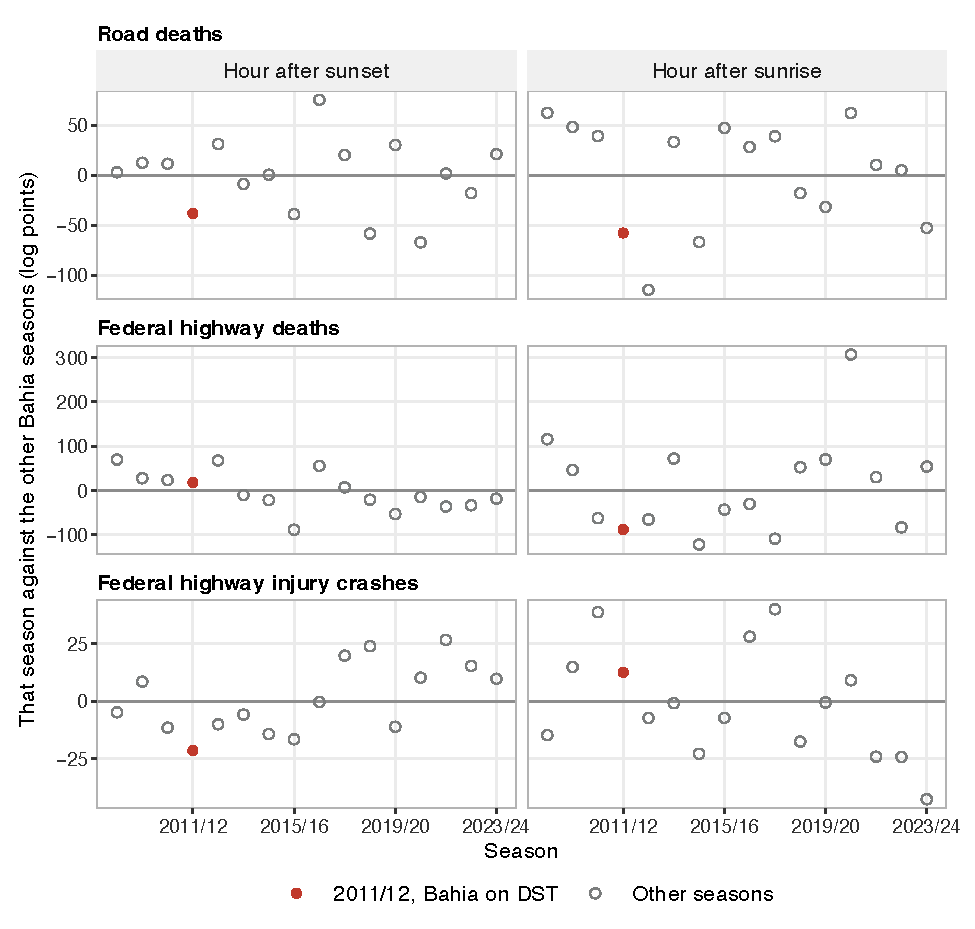
\includegraphics{fig_bahia.pdf}
  \caption{Bahia, the One Season It Had Daylight Saving Time}
  \label{fig:bahia}
  \begin{figurenotes}[Notes]
  Bahia had DST in 2011/12 only. Each point compares one Bahia season with all its other seasons, against the control states, summer window against off-season, in the hour after standard-time sunset (left) or sunrise (right). The main result predicts the 2011/12 point to be the lowest on the left and the highest on the right.
  \end{figurenotes}
  \begin{figurenotes}[Sources]
  \citet{datasus2025sim}; \citet{prf2025dados}.
  \end{figurenotes}
\end{figure}

Bahia, excluded from the main sample, had DST in a single summer, 2011/12. That summer its hour 0 was light, and in every other summer it was dark, so the main result predicts that Bahia's hour 0 had unusually few events in 2011/12. The first stage is clear: officers recorded 68 percent of Bahia's crashes in hour 0 as dusk or night in 2011/12, against 93 to 100 percent in every other season. % bahia_switch.rds, first_stage.
Tocantins, which had DST only in 2012/13, is too small for the same check: its hour 0 had about 9 federal highway injury crashes and 2 federal highway deaths per summer, against 57 and 13 in Bahia, so a single season's estimate could not be distinguished from noise. % PRF injury crashes and deaths in evening hour 0, summer window, 2008/09-2023/24: TO 8.8 and 2.0, BA 57.1 and 13.2 per season.
Figure~\ref{fig:bahia} ranks the 2011/12 estimate among Bahia's 16 seasons for each outcome. In the evening, federal highway injury crashes are the lowest of the 16 ($-21.4$ log points), road deaths the fourth lowest and federal highway deaths the eleventh lowest. In the morning the prediction fails: road deaths and federal highway deaths in 2011/12 rank third lowest, and injury crashes twelfth lowest. With one state and one season, the lowest rank of 16 corresponds to a one-sided p-value of about 0.06. We show all six comparisons as a check of sign, not as an estimate.

\subsection{Assault deaths}

\begin{figure}[tbp]
  \centering
  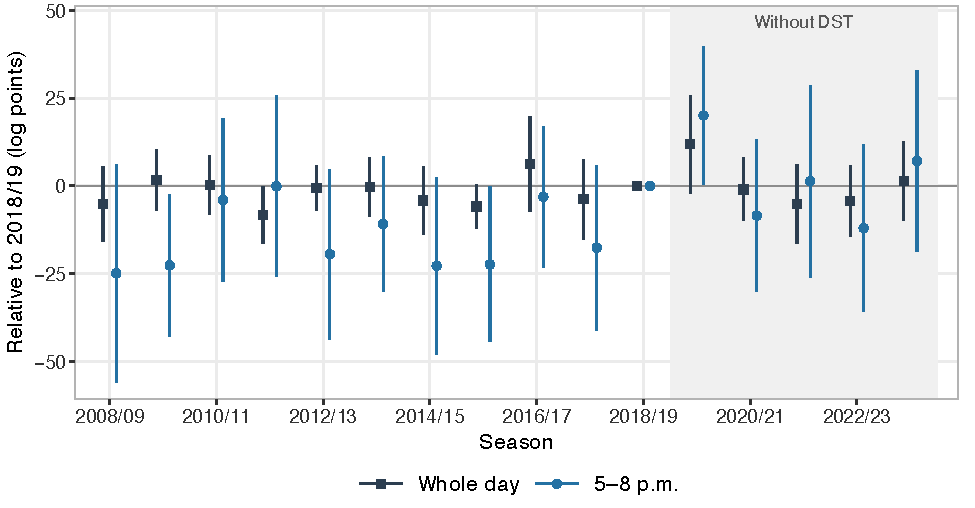
\includegraphics{fig_assault.pdf}
  \caption{Assault Deaths, Season by Season}
  \label{fig:assault}
  \begin{figurenotes}[Notes]
  Deaths from assault (ICD-10 X85--Y09) in any place, by clock time of death. Equation~(\ref{eq:main}) by season as in Figure~\ref{fig:event-study}, for the whole day and for 5 to 8 p.m.\ clock time. 95 percent confidence intervals, standard errors clustered by state.
  \end{figurenotes}
  \begin{figurenotes}[Source]
  \citet{datasus2025sim}.
  \end{figurenotes}
\end{figure}

Ambient light also affects crime \citep{doleac2015under, dominguez2023crime}, so we examined deaths from assault with the same design. They show no signature of light (Figure~\ref{fig:assault}). The whole-day triple difference is 2.4 log points (1.7), and $-0.5$ (1.5) without 2019/20, the one season in which the coefficients jump. Between 8 a.m.\ and 5 p.m., hours whose light did not change, the estimate (7.0, 2.6) is of the same order as between 5 and 8 p.m.\ (15.2, 5.0). % assault_trends.rds, results.
A change in violence concentrated in one season and spread across the day is not an effect of light, and the paper does not study assault deaths further. The triple difference can thus find changes after 2019 in hours whose light did not change; for road deaths, Panel D of Table~\ref{tab:robustness} finds none.
